% 8. Wersja na wąski ekran
\section{Wersja na wąski ekran}\label{sec:waski}

\begin{instrukcja}[wymagane]
Jak interfejs zachowuje się na telefonie albo przy zwężonym oknie: co się przestawia, co znika, co
zastępujecie czym (Wykład 4: Pionowy Stos, Dolny Pasek Nawigacyjny, duże cele dotykowe). Dodajcie
zrzuty tego samego ekranu w wersji szerokiej i wąskiej.
\end{instrukcja}

\begin{table}[H]\centering
\caption{Zmiany układu na wąskim ekranie}\label{tab:waski}
\begin{tabularx}{\linewidth}{@{}p{3.2cm}LL@{}}
\naglowektabeli \nt{Element} & \nt{Szeroki ekran} & \nt{Wąski ekran (np. poniżej 768 px)} \\
nawigacja & boczny pasek po lewej & Dolny Pasek Nawigacyjny (3 cele po 1/3 szerokości, 48\,px) \\
lista i szczegóły & Wybór Dwupanelowy & Uszczegółowienie W Jednym Oknie (osobny ekran) \\
filtr przedmiotu & przyciski-pigułki & natywna lista wyboru (jedna linia, systemowy wybierak) \\
ekran startowy & treść w kolumnie do 60\,rem & Pionowy Stos, przycisk „Dodaj termin” na całą szerokość \\
karty terminów & tytuł i liczba dni w jednym wierszu & długi tytuł zawija się, liczba dni przechodzi pod spód \\
\bottomrule
\end{tabularx}
\end{table}

\begin{figure}[H]\centering
\begin{minipage}[b]{0.62\linewidth}\centering
  \IfFileExists{obrazy/szeroki.png}{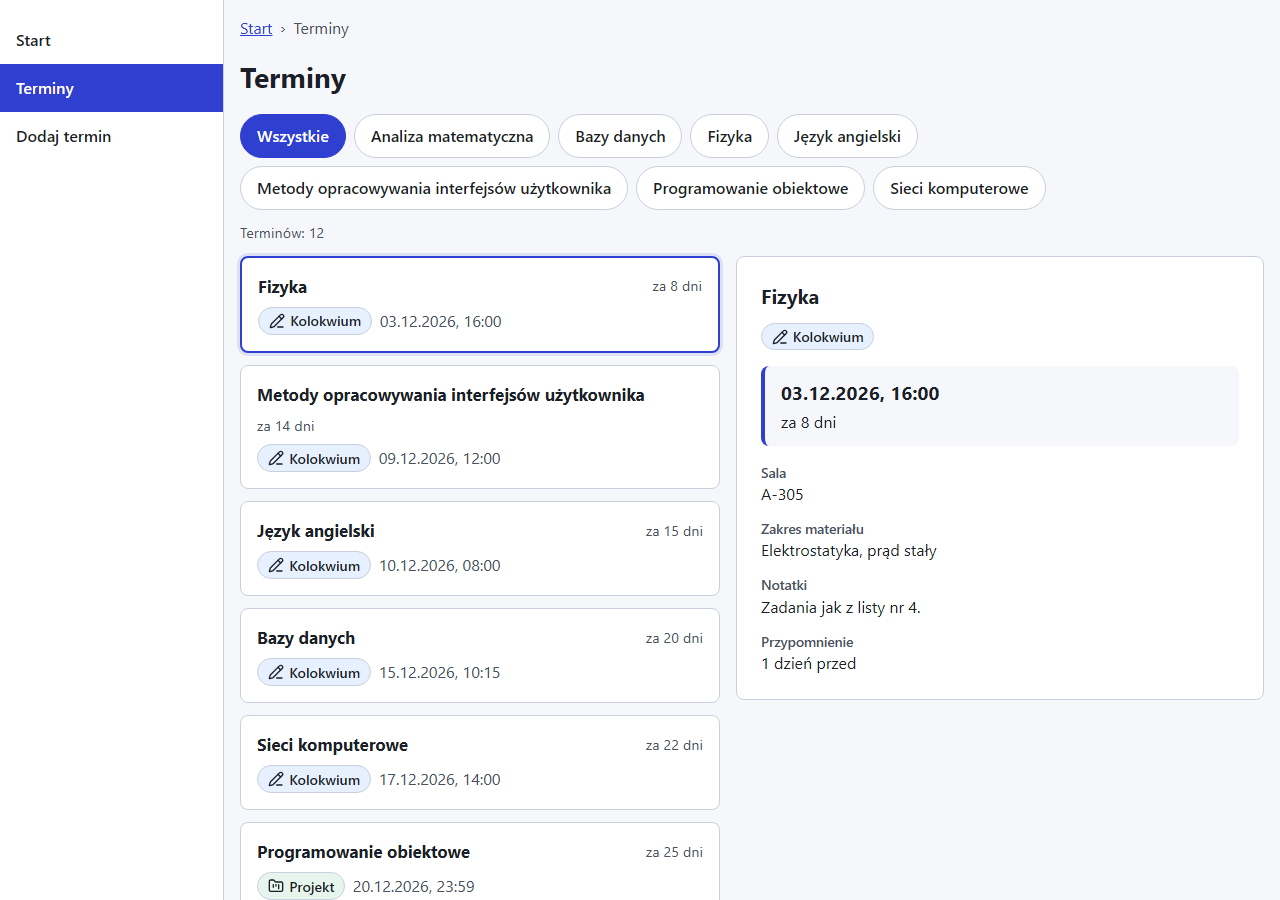
\includegraphics[width=\linewidth]{obrazy/szeroki.png}}{%
  \tikz\node[draw=dkramka,dashed,fill=dkjasny,minimum width=\linewidth,
    minimum height=5.2cm,font=\small\color{dkszary},align=center]{szeroki ekran\\\texttt{obrazy/szeroki.png}};}
\end{minipage}\hfill
\begin{minipage}[b]{0.3\linewidth}\centering
  \IfFileExists{obrazy/waski.png}{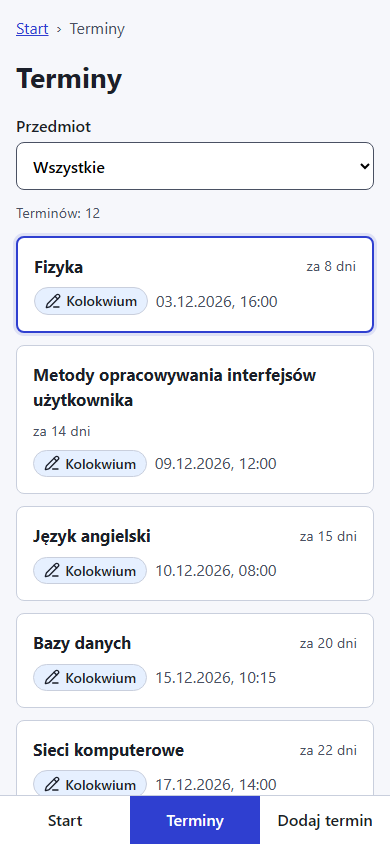
\includegraphics[width=\linewidth]{obrazy/waski.png}}{%
  \tikz\node[draw=dkramka,dashed,fill=dkjasny,minimum width=\linewidth,
    minimum height=5.2cm,font=\small\color{dkszary},align=center]{wąski ekran\\\texttt{obrazy/waski.png}};}
\end{minipage}
\caption{Ten sam ekran w wersji szerokiej i wąskiej}\label{rys:waski}
\end{figure}
